\documentclass[11pt,a4paper]{article}

\usepackage[margin=2.2cm]{geometry}
\usepackage[T1]{fontenc}
\usepackage{lmodern}
\usepackage{microtype}
\usepackage{amsmath}
\usepackage{graphicx}
\usepackage{booktabs}
\usepackage{subcaption}
\usepackage{xcolor}
\usepackage{enumitem}
\usepackage[colorlinks=true,linkcolor=blue!50!black,urlcolor=blue!50!black,citecolor=blue!50!black]{hyperref}

\graphicspath{{../images/}}
\setlist{itemsep=2pt,topsep=4pt}

\title{\textbf{Lane Detection for Autonomous Vehicles\\using Classical Computer Vision}}
\author{Piyush Anand\\\small Indian Institute of Technology Hyderabad\\\small\texttt{cs25mtech12009@iith.ac.in}}
\date{\today}

\begin{document}
\maketitle

\begin{abstract}
We present a real-time lane detection system built only from classical computer vision
operations in OpenCV. Each frame is corrected for lens distortion, filtered with a
combination of Sobel-gradient and HLS-colour thresholds, and warped to a bird's-eye view.
A sliding-window search then locates the two lane lines, which we model as second-order
polynomials and smooth over time. From the fitted lines the system estimates the road's
radius of curvature, classifies the road as straight or curving left or right, and measures
how far the vehicle sits from the lane centre. It then turns these estimates into simple
steering guidance. The pipeline runs at about 16 frames per second on a desktop CPU and
tracks lanes reliably on daytime highways. We also document where it fails: fog, night,
unmarked roads and zebra crossings.
\end{abstract}

\section{Introduction}
Lane keeping is one of the basic functions of advanced driver-assistance systems (ADAS)
and of autonomous driving. A vehicle has to know where its lane is to warn a driver who is
drifting or to steer on its own. Deep networks give the best accuracy today, but a
classical pipeline is still useful. It is transparent, needs no training data, runs on
modest hardware, and every intermediate stage can be inspected.

Our first prototype used Canny edges and the Hough transform, which detects only straight
line segments. It failed on curved roads, where lane markings bend and lens distortion
bends them further. The system described here replaces it with camera calibration, a
perspective transform and polynomial lane models, which handle curves.

\section{Method}
Figure~\ref{fig:stages} shows the pipeline. Every input frame is scaled to
$1280\times720$ (the resolution of the calibration camera) and processed at half that
resolution.

\begin{figure}[t]
  \centering
  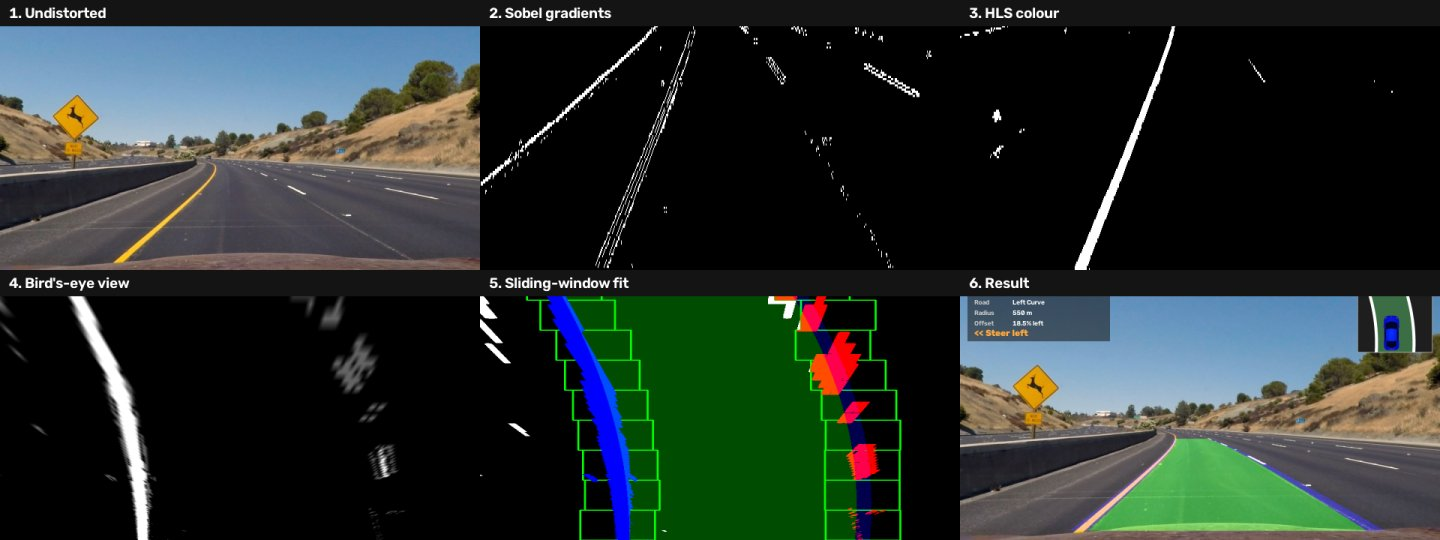
\includegraphics[width=\linewidth]{pipeline_stages.jpg}
  \caption{Pipeline stages on a left-curving highway: (1) undistorted frame,
  (2) combined Sobel mask, (3) HLS colour mask, (4) bird's-eye view,
  (5) sliding windows and fitted lanes, (6) final output with status panel and mini map.}
  \label{fig:stages}
\end{figure}

\subsection{Camera calibration}
Wide-angle lenses bend straight lines near the image border. We estimate the camera matrix
$K$ and the distortion coefficients from twenty photographs of a $9\times6$ chessboard,
using OpenCV's chessboard corner detector and \texttt{calibrateCamera}. The result is
cached, so calibration runs only once, and every frame is undistorted before any further
processing.

\subsection{Thresholding}
We process only a region of interest: the band of rows that contains the road. Two masks
are built from it.

\paragraph{Gradient mask.} On the red channel $R$, which shows both white and yellow paint
strongly, we compute Sobel derivatives $G_x$ and $G_y$, the gradient magnitude
$\sqrt{G_x^2+G_y^2}$ and the gradient direction $\theta=\arctan(|G_y|/|G_x|)$. Each is
rescaled to $[0,255]$ and thresholded. We keep a pixel if
\begin{equation}
  (G_x \wedge |\nabla| \wedge \theta) \;\vee\; (G_x \wedge G_y),
\end{equation}
which favours steep, near-vertical edges such as lane markings.

\paragraph{Colour mask.} In HLS space, saturation picks out painted markings well in
sunlight, and hue with lightness helps where markings lie in shadow. A pixel is kept if
$(S \wedge \neg L) \vee (\neg S \wedge H \wedge L)$, with the thresholds listed in
Table~\ref{tab:params}.

\subsection{Perspective transform}
We map a trapezoid on the road to a rectangle with \texttt{cv2.getPerspectiveTransform},
giving a $720\times720$ bird's-eye view. In this view, lane lines are close to parallel,
and their curvature can be measured directly.

\subsection{Lane search and fitting}
\paragraph{Blind search.} On the first frame, or after the lane is lost, we sum the lower
half of the warped mask column by column. The two histogram peaks, one in each half of the
image, give the starting $x$ positions of the lane lines. Nine windows, each
$\pm56$\,px wide, then climb the image. Each window re-centres on the mean $x$ of its
pixels whenever it contains more than 50 of them.

\paragraph{Guided search.} On later frames we search only within $\pm56$\,px of the
previous frame's curves, which is faster and more robust.

\paragraph{Model.} Each line is fitted as $x = ay^2 + by + c$. To suppress jitter, the
curves from the last ten frames are averaged and refitted. If the lane width varies too
much along the image (standard deviation $>80$\,px), the next frame falls back to a blind
search. If too few pixels are found, the last good fit is reused.

\subsection{Road geometry}
We convert pixels to metres assuming a 3.7\,m lane (the Indian standard) and a 30\,m
visible road length. The radius of curvature at the vehicle's position $y_0$ is
\begin{equation}
  R = \frac{\left(1 + (2ay_0 + b)^2\right)^{3/2}}{|2a|}.
\end{equation}
The road is classified as \emph{straight} when $R>1500$\,m and the lines lean by less than
100\,px from bottom to top. It is classified as a \emph{left} or \emph{right curve} when
$R$ is small and the lean is clearly to one side. Otherwise the previous classification is
kept. The lateral offset is the distance between the lane centre and the image centre,
expressed as a percentage of half the lane width. The classification drives the on-screen
guidance: \emph{steer left}, \emph{steer right} or \emph{keep straight}.

\begin{table}[t]
  \centering
  \small
  \begin{tabular}{@{}ll@{\qquad}ll@{}}
    \toprule
    Parameter & Value & Parameter & Value \\
    \midrule
    Sobel $x$ & 35--100 & Hue $H$ & 10--100 \\
    Sobel $y$ & 30--255 & Lightness $L$ & 0--60 \\
    Magnitude & 30--255 & Saturation $S$ & 85--255 \\
    Direction & 0.7--1.3 rad & Sliding windows & 9 $\times$ $\pm$56\,px \\
    Smoothing & 10 frames & Re-search if width std. & $>80$\,px \\
    \bottomrule
  \end{tabular}
  \caption{Main parameters.}
  \label{tab:params}
\end{table}

\section{Implementation}
The system is a small Python package, \texttt{lane\_detection}, that depends only on
OpenCV and NumPy. A stateful \texttt{LanePipeline} object processes consecutive frames and
returns the annotated image, the road status and every intermediate stage. A command-line
interface processes images, video files or a webcam stream:
\begin{center}
\texttt{python -m lane\_detection video data/videos/file2.mp4 -o out.mp4}
\end{center}
Its \texttt{--debug} flag renders the stage grid of Figure~\ref{fig:stages}, which is
useful when tuning thresholds. Unit tests cover straight and curved roads, blank frames,
recovery after a lost lane and inputs of arbitrary size.

\section{Results}
On the eight standard highway test images the lane is found in every case. The two
straight images are classified as straight and centred to within 3\,\%, and the clearly
curving images are labelled with the correct direction. Two gently curving images fall
between the straight and curve thresholds and are reported as \emph{unknown} direction,
although the lane itself is drawn correctly. On the daytime highway videos the lane is
tracked continuously, including under overpasses and past overtaking cars. End to end,
including video decoding and encoding, the pipeline runs at about 16 frames per second on
a desktop CPU.

\begin{figure}[t]
  \centering
  \begin{subfigure}{0.325\linewidth}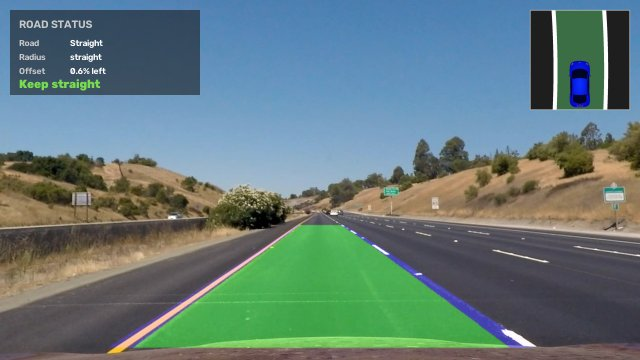
\includegraphics[width=\linewidth]{results/straight.jpg}\caption{Straight}\end{subfigure}
  \begin{subfigure}{0.325\linewidth}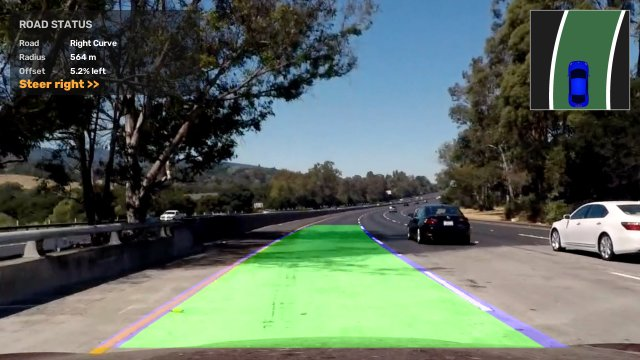
\includegraphics[width=\linewidth]{results/right_curve.jpg}\caption{Right curve}\end{subfigure}
  \begin{subfigure}{0.325\linewidth}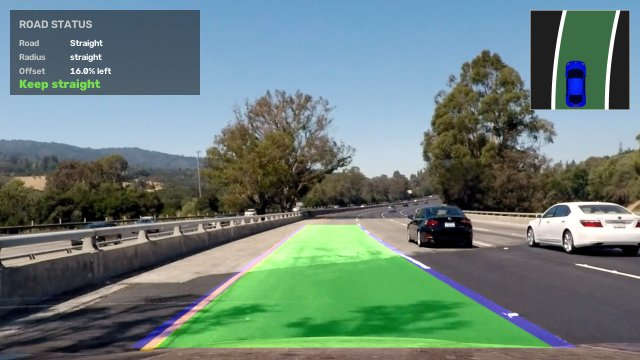
\includegraphics[width=\linewidth]{results/shadows.jpg}\caption{Shadows}\end{subfigure}\\[4pt]
  \begin{subfigure}{0.325\linewidth}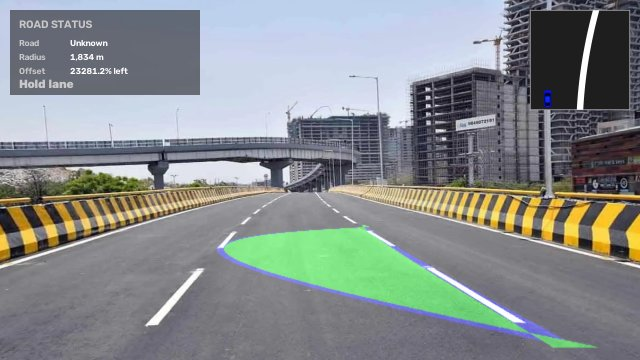
\includegraphics[width=\linewidth]{results/bridge.jpg}\caption{Bridge}\end{subfigure}
  \begin{subfigure}{0.325\linewidth}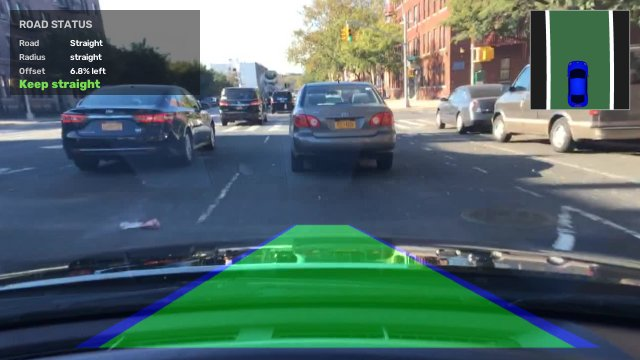
\includegraphics[width=\linewidth]{results/city_traffic.jpg}\caption{City traffic}\end{subfigure}
  \begin{subfigure}{0.325\linewidth}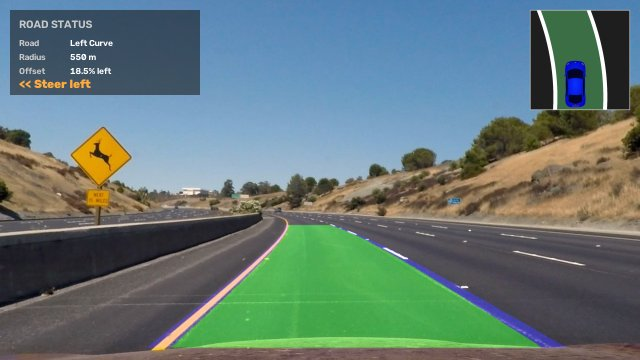
\includegraphics[width=\linewidth]{results/left_curve.jpg}\caption{Left curve}\end{subfigure}
  \caption{Scenes where the lane is detected.}
  \label{fig:good}
\end{figure}

\section{Limitations}
Figure~\ref{fig:hard} shows typical failures.
\begin{itemize}
  \item \textbf{Zebra crossings} produce strong vertical gradients that the sliding
        windows lock onto.
  \item \textbf{Unmarked roads} (sand, rural tracks) give the thresholds nothing to find,
        so the fit follows the road edge or noise.
  \item \textbf{Fog, rain and night} lower contrast. Fixed thresholds then keep too few
        pixels, or too many from glare and reflections.
  \item \textbf{Camera placement.} The perspective transform assumes a forward-facing
        camera at a fixed height. Other mountings, or portrait video, distort the
        bird's-eye view.
\end{itemize}

\begin{figure}[t]
  \centering
  \begin{subfigure}{0.24\linewidth}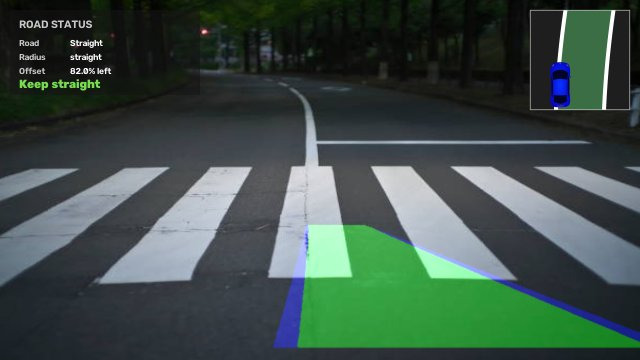
\includegraphics[width=\linewidth]{results/zebra_crossing.jpg}\caption{Zebra crossing}\end{subfigure}
  \begin{subfigure}{0.24\linewidth}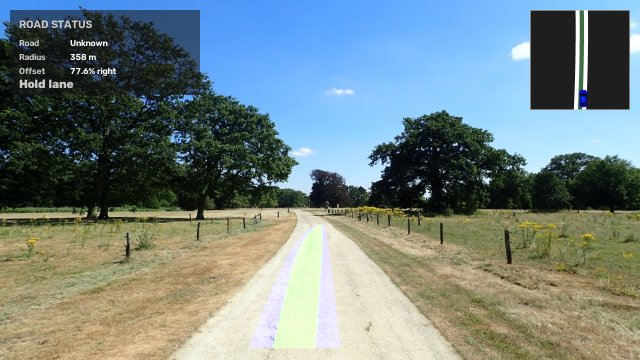
\includegraphics[width=\linewidth]{results/unmarked_road.jpg}\caption{Unmarked road}\end{subfigure}
  \begin{subfigure}{0.24\linewidth}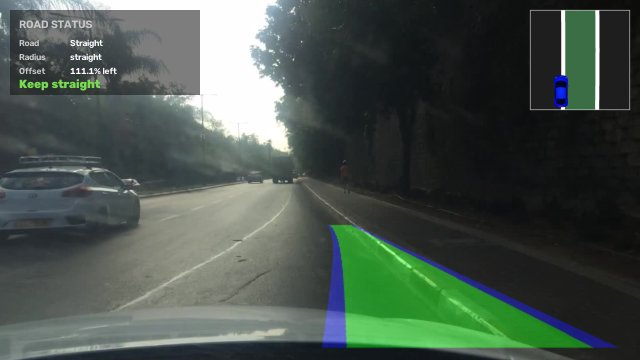
\includegraphics[width=\linewidth]{results/fog.jpg}\caption{Fog}\end{subfigure}
  \begin{subfigure}{0.24\linewidth}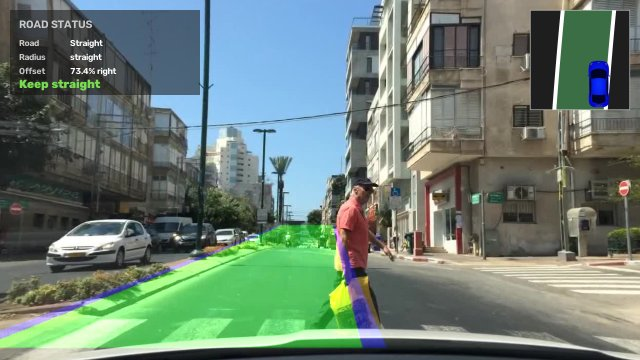
\includegraphics[width=\linewidth]{results/pedestrian.jpg}\caption{Pedestrian}\end{subfigure}
  \caption{Failure cases.}
  \label{fig:hard}
\end{figure}

\section{Conclusion and future work}
Calibration, combined gradient and colour thresholds, a bird's-eye warp and polynomial
lane models together give a lane detector that is fast, interpretable, and accurate on
curved as well as straight highways. It also provides curvature, offset and steering
guidance. To handle adverse weather, night driving and unmarked urban roads, we plan to add
adaptive (per-frame) thresholds, contrast enhancement such as CLAHE, and a lightweight
learned segmentation model. The segmentation model would replace the hand-tuned masks
while keeping the geometric back end.

\end{document}
